\section{Evaluation} \label{eval}

% To evaluate the effectiveness of each component in our algorithm design, we introduce three variants of our algorithm: BA-MBRL, BA-MCTS, and BA-MCTS-SL. (1) Existing offline MBRL methods leverage learned world models as surrogate simulators, applying reward penalties to collected transitions and employing standard online RL algorithms (e.g., SAC (\cite{DBLP:conf/icml/HaarnojaZAL18})) to learn a policy. BA-MBRL follows this approach but models the problem as a BAMDP, with environment transitions defined by Equations (\ref{bamdp-mdp}) and (\ref{b'}) and the reward penalty given by Equation (\ref{p-rwd}). BA-MBRL is designed to evaluate the effectiveness of Bayesian RL. (2) Building on BA-MBRL, BA-MCTS introduces Continuous BAMCP (Algorithm \ref{alg:2}) to plan at decision points, rather than inferring directly from the policy, to generate trajectories for downstream SAC. BA-MCTS demonstrates the impact of deep search on policy learning. (3) BA-MCTS-SL, described in Algorithm \ref{alg:3}, replaces the policy learning algorithm in BA-MCTS from policy gradient methods (as in SAC) with supervised learning (SL). By comparing these two approaches, we aim to determine which method offers a more efficient policy update mechanism, particularly for continuous control tasks.

To evaluate the effectiveness of each component in our algorithm design, we introduce three variants: (1) \textbf{BA-MBRL} leverages learned world models as surrogate simulators, applying reward penalties to collected transitions and using standard online RL algorithms (e.g., SAC (\cite{DBLP:conf/icml/HaarnojaZAL18})) to learn a policy. While following existing offline MBRL methods, it models the problem as a BAMDP (rather than an MDP), with environment transitions defined by Equations (\ref{bamdp-mdp}) and (\ref{b'}) and the reward penalty by Equation (\ref{p-rwd}), and is designed to evaluate the effectiveness of Bayesian RL. (2) \textbf{BA-MCTS} builds on BA-MBRL by introducing Continuous BAMCP (Algorithm \ref{alg:2}) to plan at decision points, rather than inferring directly from the policy, to generate trajectories for downstream SAC, demonstrating the impact of deep search on policy learning. (3) \textbf{BA-MCTS-SL}, described in Algorithm \ref{alg:3}, replaces the policy learning algorithm in BA-MCTS from policy gradient methods (as in SAC) with supervised learning (SL), allowing us to compare which approach offers a more efficient policy update mechanism, particularly for continuous control tasks.
 
\begin{table}[t]
\scriptsize
\centering
\begin{tabular}{c|c|c|c|c|c|c|c|c}
\hline
{\makecell{Data Type}} & {Environment} & {\makecell{BA-MCTS \\ -SL (ours)}} & {\makecell{BA-MCTS \\ (ours)}} & {\makecell{BA-MBRL \\ (ours)}} & {Optimized} & {COMBO} & {MOReL} & {MOPO}\\
\hline 
\hline
{random} & {HalfCheetah} & {29.20 $\pm$ 2.00} & {36.23 $\pm$ 1.04} & {32.76 $\pm$ 1.16} & {31.7} & {\textbf{38.8}} & {25.6} & {35.4} \\
{random} & {Hopper} & {33.83 $\pm$ 0.10} & {31.56 $\pm$ 0.12} & {31.47 $\pm$ 0.03} & {12.1} & {17.9} & {\textbf{53.6}} & {11.7} \\
{random} & {Walker2d} & {21.89 $\pm$ 0.07} & {21.59 $\pm$ 0.32} & {21.45 $\pm$ 0.53} & {21.7} & {7.0} & {\textbf{37.3}} & {13.6} \\
\hline
{medium} & {HalfCheetah} & {70.47 $\pm$ 3.52} & {\textbf{75.84} $\pm$ 3.81} & {56.54 $\pm$ 5.20} & {45.7} & {54.2} & {42.1} & {42.3} \\
{medium} & {Hopper} & {97.75 $\pm$ 7.09} & {96.70 $\pm$ 14.0} & {\textbf{98.25} $\pm$ 3.42} & {69.3} & {97.2} & {95.4} & {28.0} \\
{medium} & {Walker2d} & {\textbf{82.24} $\pm$ 1.85} & {74.73 $\pm$ 3.25} & {75.41 $\pm$ 4.17} & {79.7} & {81.9} & {77.8} & {17.8} \\
\hline 
{med-replay} & {HalfCheetah} & {61.16 $\pm$ 1.60} & {\textbf{65.45} $\pm$ 0.81} & {62.50 $\pm$ 0.18} & {58.0} & {55.1} & {40.2} & {53.1} \\
{med-replay} & {Hopper} & {\textbf{106.3} $\pm$ 0.13} & {101.8 $\pm$ 3.46} & {93.91 $\pm$ 4.25} & {90.8} & {89.5} & {93.6} & {67.5} \\
{med-replay} & {Walker2d} & {92.13 $\pm$ 5.13} & {95.06 $\pm$ 2.11} & {\textbf{97.54}$\pm$ 1.93} & {65.8} & {56.0} & {49.8} & {39.0} \\
\hline 
{med-expert} & {HalfCheetah} & {80.53 $\pm$ 6.63} & {76.16 $\pm$ 10.3} & {90.52 $\pm$ 4.13} & {\textbf{104.2}} & {90.0} & {53.3} & {63.3} \\
{med-expert} & {Hopper} & {\textbf{112.2} $\pm$ 0.29} & {108.3 $\pm$ 0.22} & {107.8 $\pm$ 0.37} & {105.8} & {111.1} & {108.7} & {23.7} \\
{med-expert} & {Walker2d} & {107.7 $\pm$ 0.82} & {\textbf{110.0} $\pm$ 1.74} & {84.71 $\pm$ 0.87} & {97.1} & {103.3} & {95.6} & {44.6} \\
\hline
\hline
\multicolumn{2}{c|}{Average Score} & {\textbf{74.62}} & {74.45} & {71.06} & {65.16} & {66.83} & {64.42} & {36.67} \\
\hline 
\end{tabular}
\caption{Comparisons between the proposed algorithms and SOTA offline model-based RL methods on the D4RL benchmark suite. Each value represents the normalized score, as proposed in (\cite{DBLP:journals/corr/abs-2004-07219}), of the policy trained by the corresponding algorithm. These scores are undiscounted returns normalized to approximately range between 0 and 100, where a score of 0 corresponds to a random policy and a score of 100 corresponds to an expert-level policy. For our algorithms, we report the average score of the final ten policy learning epochs and its standard deviation across three random seeds. Results in the last four columns are taken from the original papers (\cite{DBLP:conf/iclr/LuBPOR22, DBLP:conf/nips/YuKRRLF21, DBLP:conf/nips/KidambiRNJ20, DBLP:conf/nips/YuTYEZLFM20}), respectively.} 
\label{table:1}
\end{table}

We first evaluate our algorithms on a widely-used continuous control benchmark for offline RL methods -- D4RL MuJoCo (\cite{DBLP:journals/corr/abs-2004-07219}). The evaluation results for three types of robotic agents, each with offline datasets of four different qualities, are presented in Table \ref{table:1}. (1) Compared to SOTA offline MBRL methods, our algorithms achieve superior performance on nine out of twelve tasks. In terms of average performance, BA-MBRL significantly outperforms the baselines, demonstrating the effectiveness of using BAMDPs to handle model uncertainties in offline MBRL. (2) Both BA-MCTS and BA-MCTS-SL further improve upon BA-MBRL, highlighting the enhancement brought by deep search in policy learning. Notably, we apply Continuous BAMCP to only 10\% of states when collecting training trajectories, while for the remaining states, we sample actions directly from the policy, i.e., $a \sim \pi(\cdot|s)$. Increasing the search ratio could further enhance policy performance at the cost of increased computation. (3) BA-MCTS-SL performs similarly to BA-MCTS, validating the effectiveness of both policy update mechanisms. However, BA-MCTS-SL struggles on Walker2d, where a warm-up training phase (using BA-MBRL) is required to establish a better initial policy. On the other hand, the advantage of the SL-based policy update is evident in the training plots of our algorithms in Figure \ref{fig:3}, where BA-MCTS-SL exhibits much smoother learning curves compared to the other two algorithms, indicating greater robustness in model selection. (4) We further compare our algorithms with model-free offline policy learning methods, as shown in Appendix \ref{ComMF}. The performance improvement is even greater than that over model-based methods, highlighting the necessity of model-based learning. Particularly, when data quality is low, merely mimicking or staying close to the behavior policy would result in an underperforming policy. (5) We provide an ablation study in Appendix \ref{ASRP} to demonstrate the necessity of incorporating the reward penalty in offline MBRL to prevent the overexploitation of inaccurate world models. Additionally, we find that the SL-based policy update is less sensitive to model inaccuracies.

\begin{figure*}[t]
\centering
\subfigure[hc-med-expert]{
\label{fig:1(a)} 
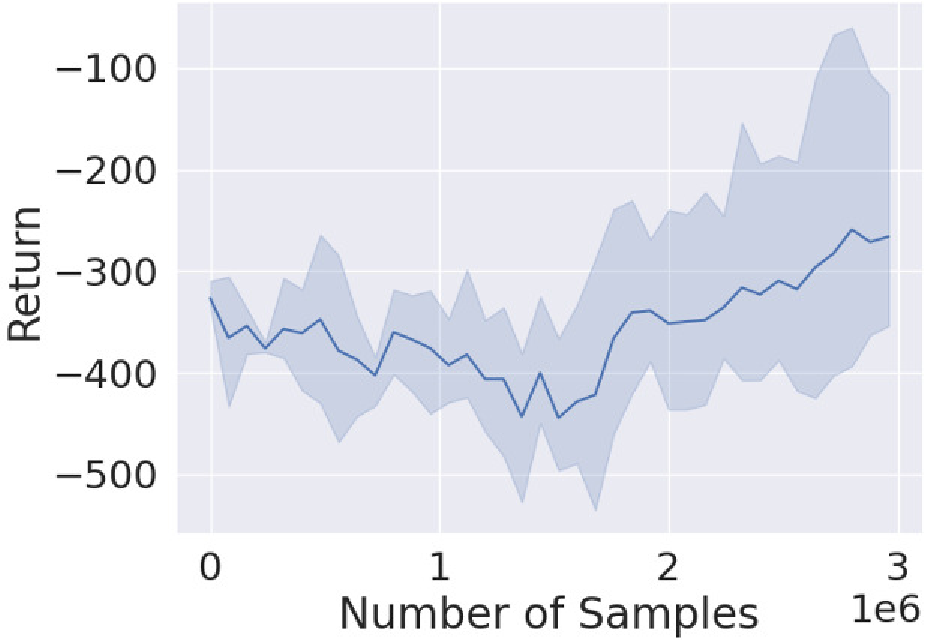
\includegraphics[width=1.5in, height=0.8in]{hc-m-exp-mz.pdf}}
\subfigure[hc-med-replay]{
\label{fig:1(b)} 
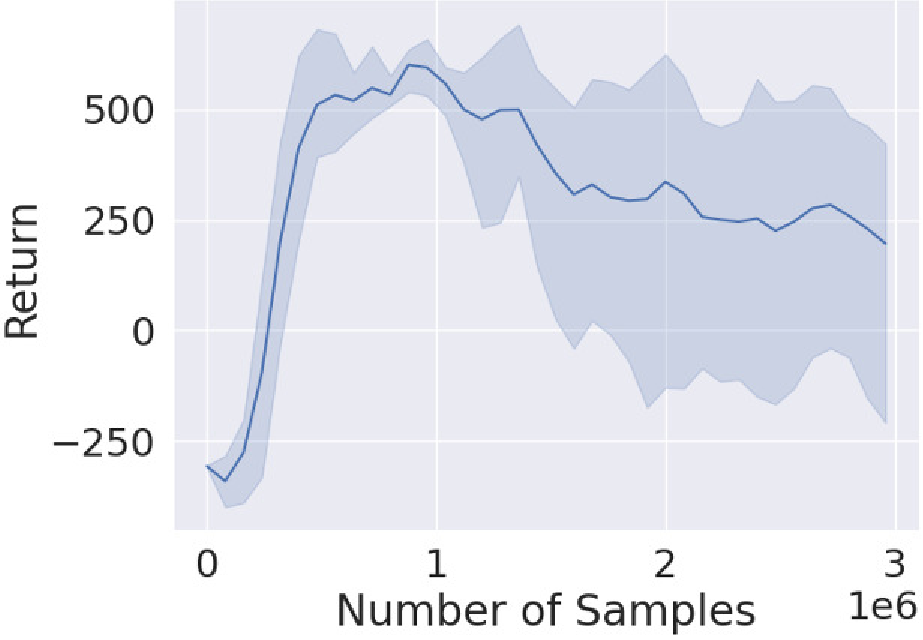
\includegraphics[width=1.5in, height=0.8in]{hc-m-rep-mz.pdf}}
\subfigure[hc-medium]{
\label{fig:1(c)} 
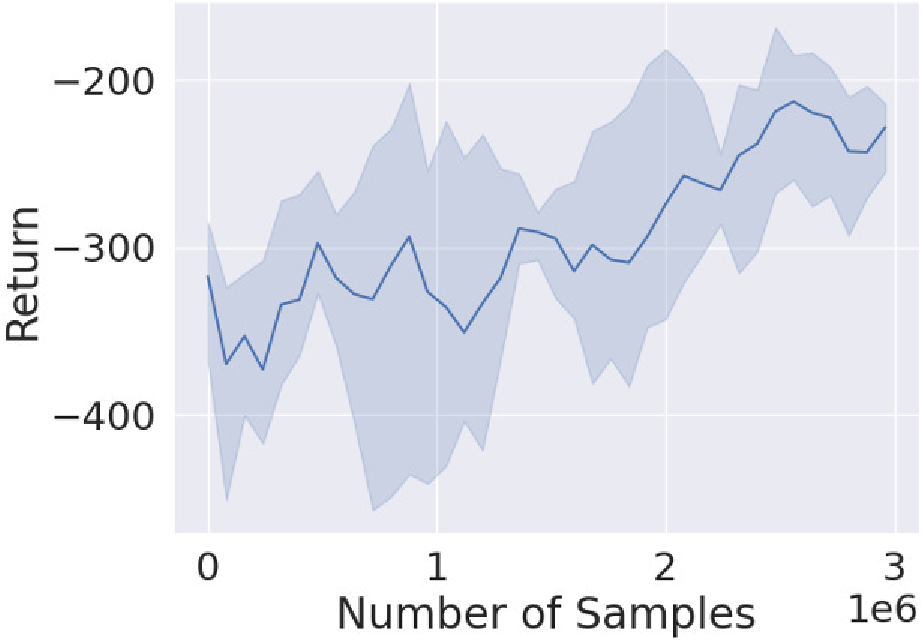
\includegraphics[width=1.5in, height=0.8in]{hc-med-mz.pdf}}
\subfigure[hc-random]{
\label{fig:1(d)} 
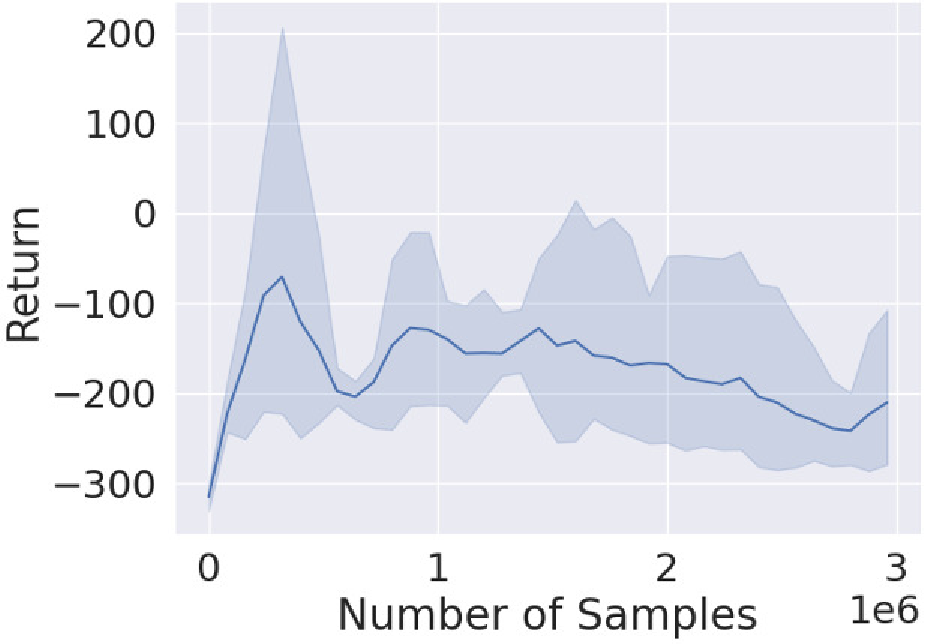
\includegraphics[width=1.5in, height=0.8in]{hc-rnd-mz.pdf}}
\subfigure[hp-med-expert]{
\label{fig:1(e)} 
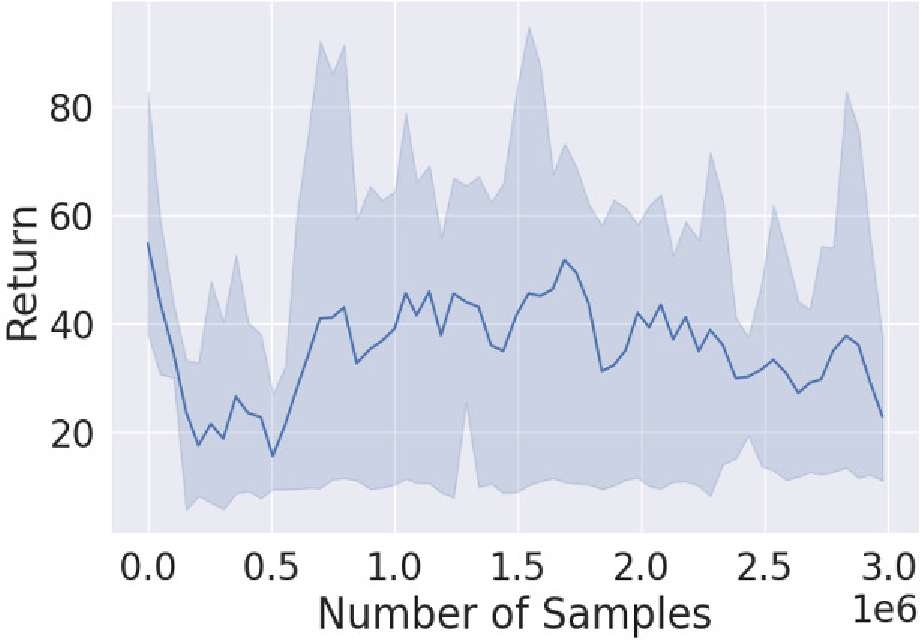
\includegraphics[width=1.5in, height=0.8in]{hp-m-exp-mz.pdf}}
\subfigure[hp-med-replay]{
\label{fig:1(f)} 
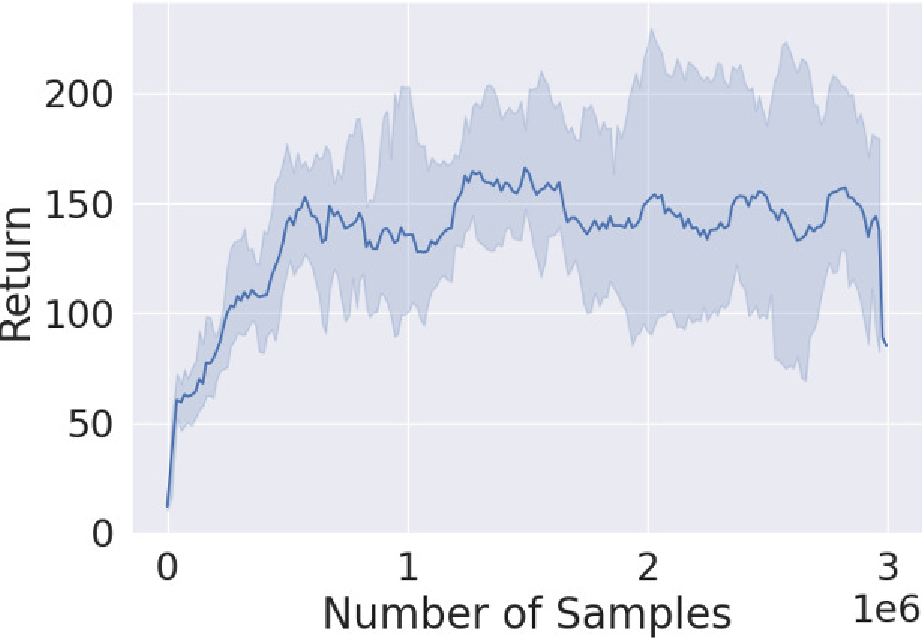
\includegraphics[width=1.5in, height=0.8in]{hp-m-rep-mz.pdf}}
\subfigure[hp-medium]{
\label{fig:1(g)} 
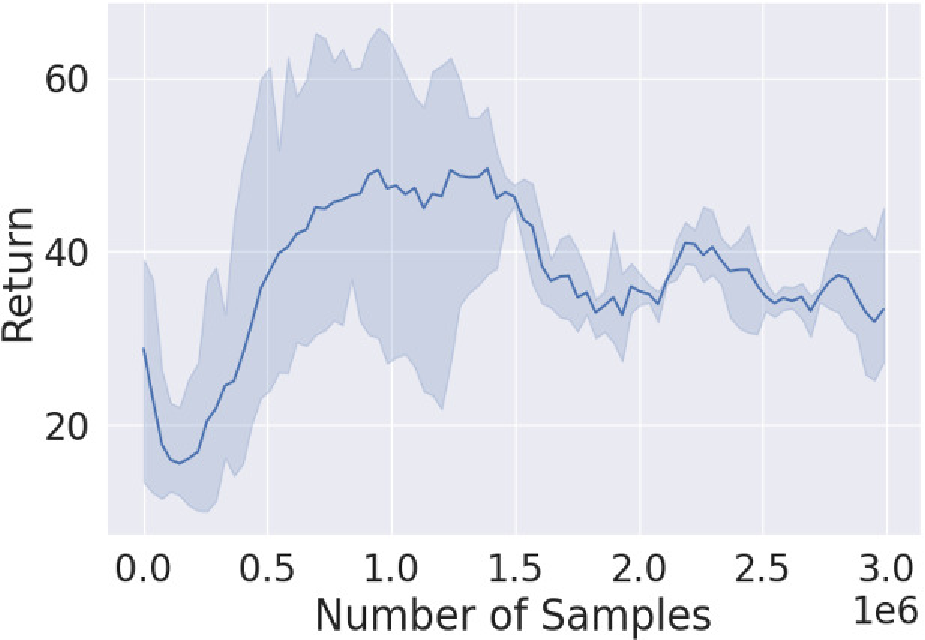
\includegraphics[width=1.5in, height=0.8in]{hp-med-mz.pdf}}
\subfigure[hp-random]{
\label{fig:1(h)} 
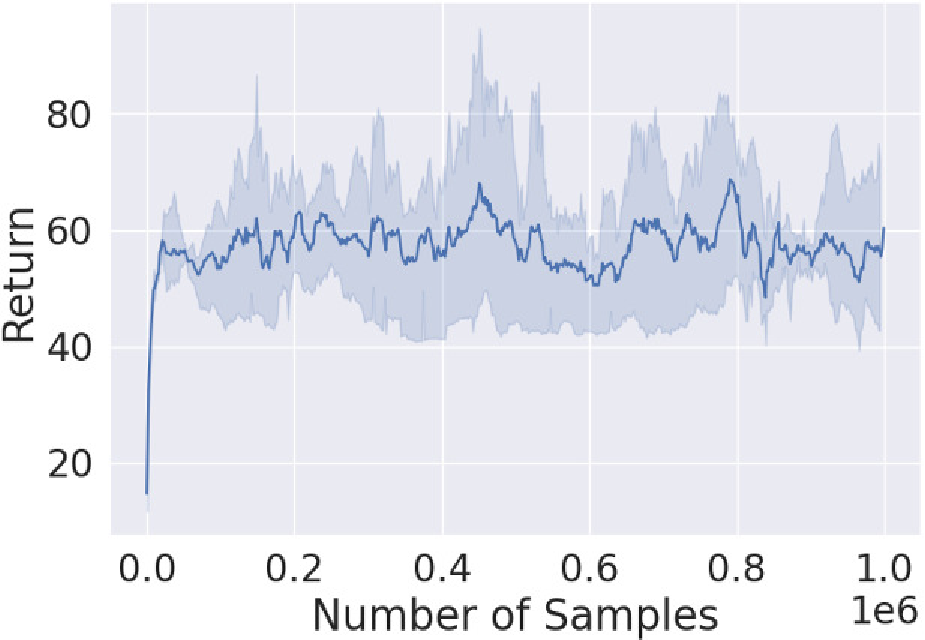
\includegraphics[width=1.5in, height=0.8in]{hp-rnd-mz.pdf}}
\subfigure[wk-med-expert]{
\label{fig:1(i)} 
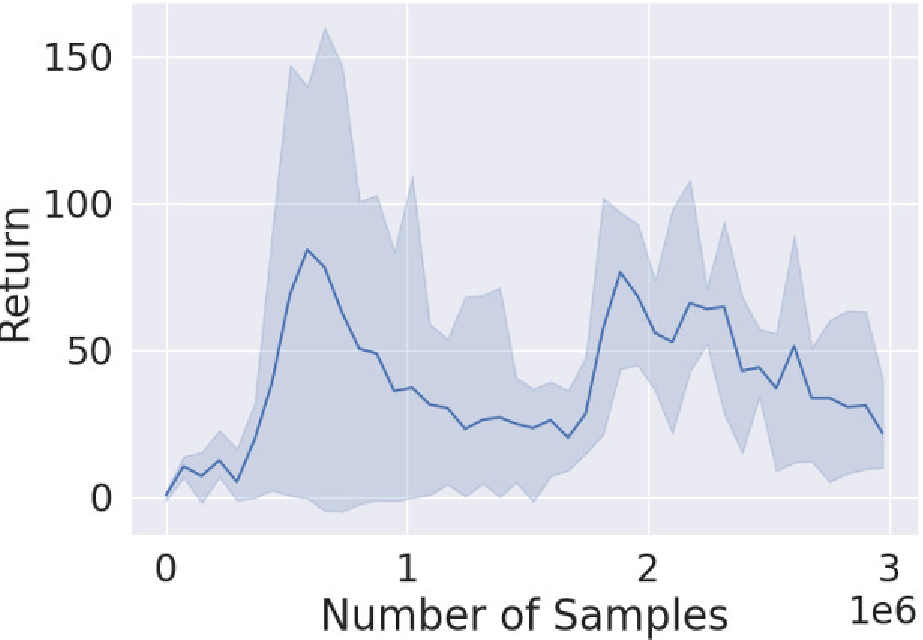
\includegraphics[width=1.5in, height=0.8in]{wk-m-exp-mz.pdf}}
\subfigure[wk-med-replay]{
\label{fig:1(j)} 
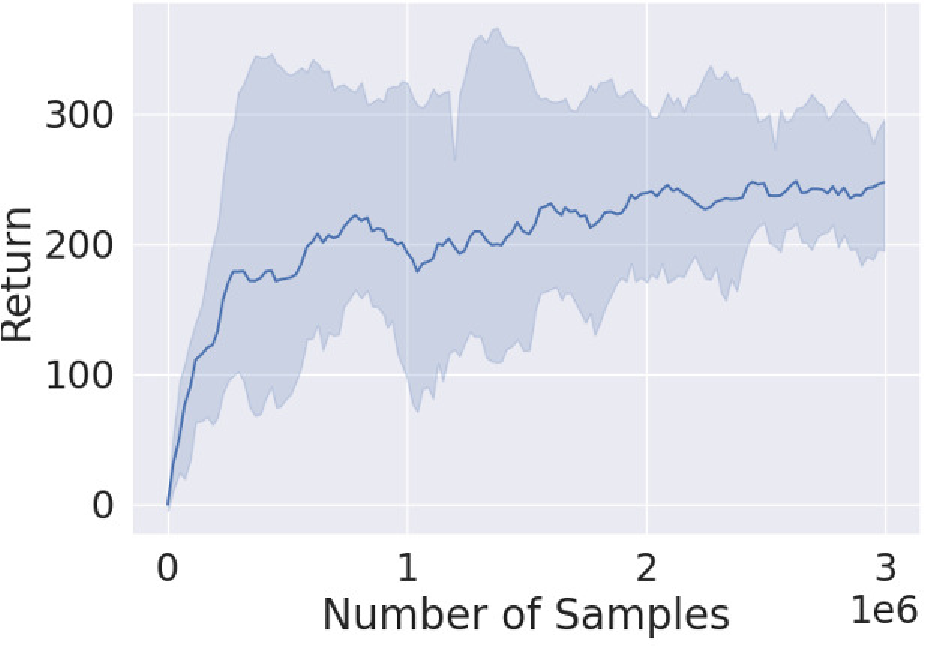
\includegraphics[width=1.5in, height=0.8in]{wk-m-rep-mz.pdf}}
\subfigure[wk-medium]{
\label{fig:1(k)} 
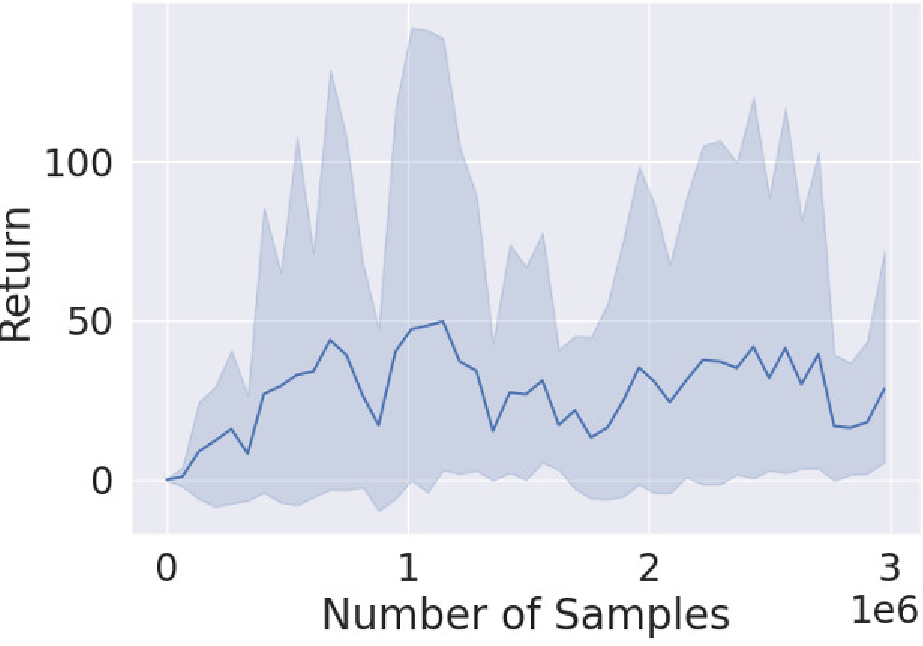
\includegraphics[width=1.5in, height=0.8in]{wk-med-mz.pdf}}
\subfigure[wk-random]{
\label{fig:1(l)} 
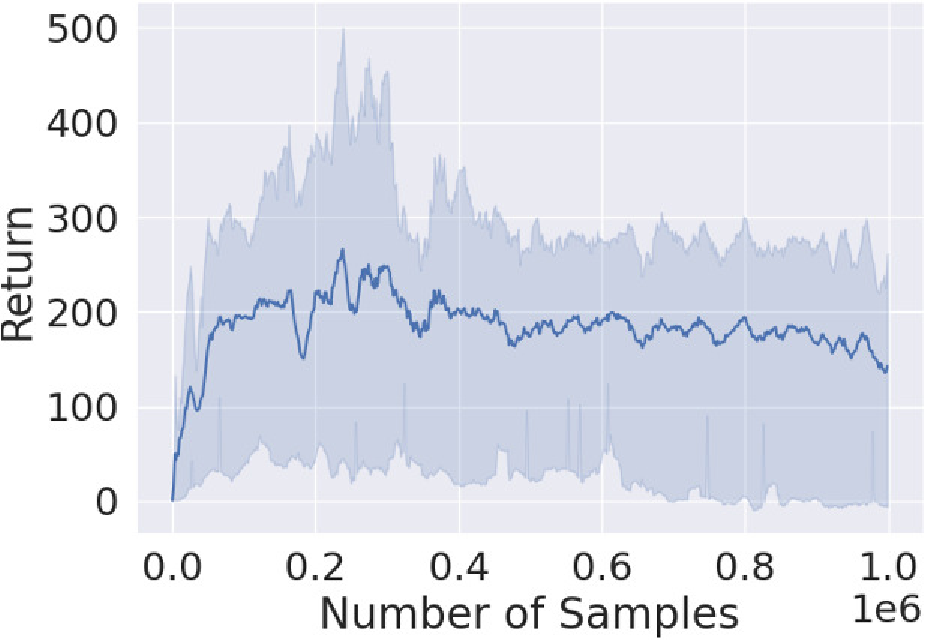
\includegraphics[width=1.5in, height=0.8in]{wk-rnd-mz.pdf}}
\caption{Performance of Sampled EfficientZero on D4RL MuJoCo tasks. The results for HalfCheetah, Hopper, and Walker2d are presented in the three rows, respectively. Each subfigure depicts the change in undiscounted episodic return as a function of the number of training samples. Experiments are repeated three times with different random seeds, with the solid line representing the mean and the shaded area indicating the 95\% confidence interval. For reference, the expert-level episodic returns for HalfCheetah, Hopper, and Walker2d are 12135, 3234.3, and 4592.3, respectively.}
\label{fig:1} 
\end{figure*}


\begin{figure}[t]
    \centering
    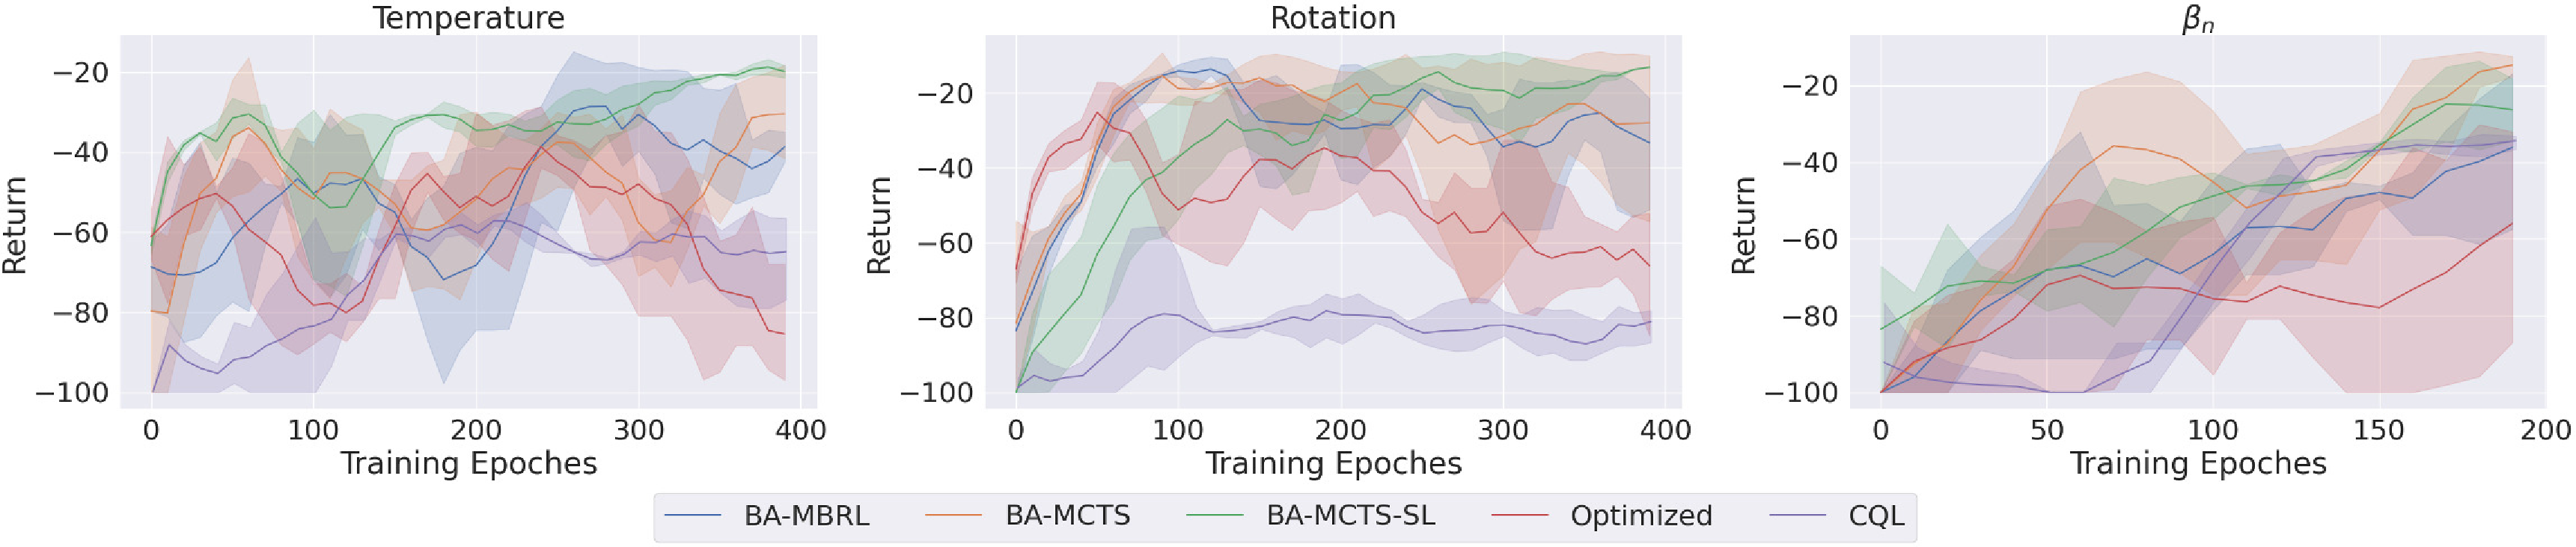
\includegraphics[width=\linewidth, height=1.5in]{nf_return-eps-converted-to.pdf} % or use height
    \caption{Evaluation results for the tokamak control tasks. The figure shows the change in episodic returns over training epochs for the proposed algorithms and baselines across three target tracking tasks in the nuclear fusion scenario. Solid lines represent the average performance, while shaded areas indicate the 95\% confidence intervals.}
    \label{fig:2}
\end{figure}

For fair comparisons and real-time execution, we do not perform test-time search and adopt the same policy architecture as the baselines, i.e., a feedforward neural network, rather than an RNN that incorporates transition history as input. These alternative designs have the potential to further improve our algorithms. For implementation, we build on the codebase of Optimized (\cite{DBLP:conf/iclr/LuBPOR22}), which thoroughly explores design choices in offline MBRL, making minimal changes to the code and hyperparameter settings\footnote{The detailed hyperparameter setups of our algorithms are provided in Appendix \ref{KeyPara}.}. Therefore, we believe the performance improvements stem from the Bayesian RL framework and deep search component. Further, both components can be seamlessly integrated with other advancements in offline MBRL, such as more accurate world model learning and improved uncertainty quantification for constructing pessimistic MDPs. 

MuZero also applies deep search to MBRL. To evaluate its performance on D4RL MuJoCo tasks, we use the open-source implementation and hyperparameter configurations of Sampled EfficientZero (\cite{DBLP:conf/nips/YeLKAG21}) provided by LightZero (\cite{DBLP:conf/nips/NiuPYLZRHLL23}). Benchmarking results from LightZero indicate that Sampled EfficientZero, equipped with a Gaussian policy, achieves the best performance on (online) MuJoCo locomotion tasks compared to other MuZero variants. To adapt Sampled EfficientZero for offline learning, we employ the reanalyse technique proposed by (\cite{DBLP:conf/nips/SchrittwieserHM21}). The evaluation results are presented in Figure \ref{fig:1}. For reference, the expert-level episodic returns (corresponding to scores of 100) for HalfCheetah, Hopper, and Walker2d are 12135, 3234.3, and 4592.3, respectively. As shown, the results are significantly worse compared to the performance of offline RL methods listed in Table \ref{table:1}, despite Sampled EfficientZero's higher computational cost (detailed in Appendix \ref{CompCost}). Notably, both Sampled EfficientZero and BA-MCTS-SL rely on supervised learning for policy improvement. However, for continuous control tasks, the agent can only sample a finite number of actions at a decision point, and the search result (e.g., $\pi_{\text{ret}}$ in Algorithm \ref{alg:2}) is a distribution over this finite set, which could be a poor approximation of the optimal action distribution. Thus, purely mimicking the search result may be less sample-efficient than policy gradient methods, as it fails to account for the continuous nature of the action space. Furthermore, world model learning is the foundation of MBRL and can be particularly challenging in \textbf{continuous control and offline learning settings}, where the state-action space is vast but training data is limited. Sampled EfficientZero integrates model learning and policy training into a single stage, which significantly increases the learning difficulty (compared to BA-MCTS-SL).

Finally, we evaluate our algorithms on three target tracking tasks in tokamak control. The tokamak is one of the most promising confinement devices for achieving controllable nuclear fusion, where the primary challenge lies in confining the plasma, i.e., an ionized gas of hydrogen isotopes, while heating it and increasing its pressure to initiate and sustain fusion reactions (\cite{1512794}). Tokamak control involves applying a series of direct actuators (e.g., neutral beam, ECH power, magnetic field) and indirect actuators (e.g., setting targets for the plasma shape and density) to confine the plasma to achieve a desired state or track a given target. This sophisticated physical process is an ideal test bed for our algorithms. Specifically, we use a well-trained data-driven dynamics model provided by \cite{DBLP:journals/corr/abs-2404-12416} as a ``ground truth" simulator for the nuclear fusion process during evaluation, and generate a dataset containing 725270 transitions using this model for offline RL. We select a reference shot (i.e., an episode of a fusion process) from DIII-D\footnote{DIII-D is a tokamak device located in San Diego, California, operated by General Atomics.}, and use its trajectories of Ion Rotation, Electron Temperature, and $\beta_n$ as targets for three tracking tasks. These are critical quantities in tokamak control, particularly $\beta_n$, which serves as an economic indicator of the efficiency of nuclear fusion. The tracking tasks have a 28-dimensional state space and a 14-dimensional action space, both continuous. Moreover, these tasks are \textbf{highly stochastic}, as the underlying dynamics model is a probabilistic neural network and each state transition is a sample from this model. For details on the simulator, and the design of the state/action spaces and reward functions, please refer to Appendix \ref{DetTCT}. We compare our algorithms with SOTA model-free and model-based offline RL methods, specifically CQL and Optimized. The learning performance on the three tracking tasks is shown in Figure \ref{fig:2}, where the x-axis and y-axis represent the training epochs and (negative) full-shot tracking errors, respectively. Our algorithms consistently outperform the baselines. Notably, the offline dataset does not include the reference shot or any similar, nearby shots. Therefore, restricting the policy to stay close to the behavior policy, as done in model-free methods, can be problematic. Also, learning dynamics models for MBRL is quite challenging in this nuclear fusion scenario. Our algorithms share the same ensemble of dynamics models with ``Optimized" for policy learning, and the comparisons can demonstrate the superiority of Bayesian RL and deep search. Figure \ref{fig:2} has been smoothed for visualization\footnote{The episodic return is plotted every 10 training epochs, with the y-axis representing the average value of a sliding window of length 5.}. We further report the average return over the final 10 training epochs in Table \ref{table:6}, and the conclusions align with those from the D4RL MuJoCo tasks, showing the robustness of our proposed algorithms.

\begin{table}[t]
\small
\centering
\begin{tabular}{c|c|c|c|c|c}
\hline
{Task} & {\makecell{BA-MCTS \\ -SL (ours)}} & {\makecell{BA-MCTS \\ (ours)}} & {\makecell{BA-MBRL \\ (ours)}} & {CQL} & {Optimized}\\
\hline 
\hline
{Temperature} & {\textbf{-21.16} $\pm$ 5.00} & {-23.83 $\pm$ 9.66} & {-29.35 $\pm$ 4.72} & {-59.62 $\pm$ 1.57} & {-83.55 $\pm$ 10.56} \\
{Rotation} & {\textbf{-14.14} $\pm$ 1.88} & {-19.07 $\pm$ 5.85} & {-31.33 $\pm$ 11.54} & {-85.48 $\pm$ 2.72} & {-71.54 $\pm$ 9.88} \\
{$\beta_{n}$} & {-37.03 $\pm$ 17.98} & {\textbf{-18.93} $\pm$ 1.75} & {-23.4 $\pm$ 10.77} & {-36.37 $\pm$ 1.17} & {-57.84 $\pm$ 10.27} \\
\hline
\hline
{Average} & {-24.11} & {\textbf{-20.61}} & {-28.03} & {-60.49} & {-70.98} \\
\hline 
\end{tabular}
\caption{Comparisons between the proposed algorithms and offline RL baselines on the target tracking tasks. For each algorithm, we report the average return of the final ten policy learning epochs and its standard deviation across three different random seeds.}
\label{table:6}
\end{table}

 % get rid of implementation tricks, do minimal changes, see the improvement brought by the search component. 

 % muzero fails, learning dyn and policy at the same stage can be very challenging, especially for complex continuous control tasks